\setchapterpreamble[u]{\margintoc}
\chapter{Servers}
\epigraph{\emph{"Simplicity, carried to an extreme, \\ becomes elegance."}}{ -- Jon Franklin}

Servers are probably one of the most misunderstood concepts for new developers. If you put ten new developers in a room, it's a pretty good bet that they've all \emph{heard} of servers. Maybe they've been exposed to them through pop culture. They've seen movies or read books where the nerdy, basement dwelling side character is approached by the charismatic protagonist to "hack into the mainframe" to stop the evil corporation and save the world.\sidenote{Note that a mainframe is just a special name for a server that is capable of performing a large amount of concurrent operations. Whether or not "hacking" into one will save the world is another question.} Or maybe they've come across the terminology at some point while learning about the fundamentals of programming, with their instructors glossing over it saying, "don't worry about this yet." Whatever the case may be, its likely that a majority of the ten new developers you have confined to a room would not be able to tell you what exactly a server does, or why. Or even more fundamentally, what \emph{is} a server? 

In a way, this lack of understanding almost serves as a hint to what a server is: a blackbox\sidenote{A blackbox is a term for an object that takes some input and transforms it into some desired output, with the user not necessarily knowing the details of how it works.} to process and retrieve information. We see this concept, \kw{abstraction}, fairly frequently in programming and Computer Science. Through abstraction, we make it far simpler for others to interact with our programs. It's a very important concept, and we'll be digging into it in detail throughout this chapter. 

This write-off of servers as blackboxes is great if we just want to use them to get some data. It makes our job much easier! In fact, you interact with servers (indirectly) every single day just by browsing the internet.\sidenote{Can you imagine if you had to be familiar with all the intricacies of servers just to watch a YouTube video?} However, when it comes time to create our own, it's important to have a deeper understanding. And that's what we aim to accomplish here! By first instilling in you an idea of the \emph{fundamental} concept of a server,\sidenote{Note that we won't go over all the low level implementation details. That's for your upper division CS classes to cover!} and later showing one possible implementation (among many), we'll break the blackbox open and expose the ideas within.

\section{Servers In General}

Put simply, a server is a computer like any other. What distingishes a regular old computer and a server is that \kw{servers are given the task of listening and responding to requests}. These tend to be requests for data or to perform some task and in general they come from other computers.\sidenote{We will see that it's not always the case that requests originate from other computers. A single computer can be both the server and the client, and you'll see that this is actually very common, particularly during the development process of a full stack application.} We call these "other" computers \kw{clients}. You can think of the interaction between a server and a client in much the same way as the interaction between a customer at a restaurant and the restaurant's staff. Just as a customer can request a glass of water, new silverware, or a half serving of Tiramisu, a client can request some function to be performed or data to be processed and returned. This brings up an important question: how do the client and server communicate? A customer at a restaurant might use English or Portuguese, but unfortunately computers aren't quite there yet. They must have some standard, agreed upon language in order to do so.

\subsection*{The Language of Requests}

In the context of clients and servers, the "language" that is typically used is \kw{HTTP}, or Hypertext Transfer Protocol.\sidenote{Note that there are other protocols that can be used, such as WebRTC, and each have their advantages. For now, let's not get into the weeds too much, but I recommend reading up on protocols if you're interested.} This protocol makes it easier for servers to parse through a client's request due to the fixed format. Take a look at the following example of a real HTTP request:

\begin{lstlisting}[language=html]
    GET / HTTP/1.1
    Host: www.example.com
    User-Agent: Mozilla/5.0
    Accept: text/html,application/xhtml+xml,application/xml;
            q=0.9,image/avif,image/webp,*/*;q=0.8
    Accept-Language: en-GB,en;q=0.5
    Accept-Encoding: gzip, deflate, br
    Connection: keep-alive
\end{lstlisting}

It may seem strange and hard to read as a human, but it is perfectly formatted for computers. We don't have to worry about the exact formatting as creating these requests is typically automated, but I do want to point out one key detail: the word \texttt{GET}. \texttt{GET} indicates to the server the particular action desired by the client, and it is one of several so called \kw{HTTP request methods}. We'll discuss these in more detail and show several examples, so don't worry if you haven't quite grasped the concept yet. For now, here are a few essential methods to be aware of \sidenote{There are methods beyond these. Check out Mozilla's \href{https://developer.mozilla.org/en-US/docs/Web/HTTP/Methods}{article} on the subject if you're interested.}: 

\begin{itemize}
    \item \texttt{GET}: indicates a request for some data
    \item \texttt{POST}: submits data to the server which often results in some side effect or change to the server's state
    \item \texttt{PUT}: submits data to the server in order to update an existing resource
    \item \texttt{DELETE}: removes some resource from the server
\end{itemize}

After receiving a well-formed request, the server will perform the specified action and create a \kw{response} to send back to the client. The format of a response is also standardized by HTTP, and here is an example:

\begin{lstlisting}[language=html]
    HTTP/1.1 200 OK
    Date: Mon, 23 May 2005 22:38:34 GMT
    Content-Type: text/html; charset=UTF-8
    Content-Length: 155
    Last-Modified: Wed, 08 Jan 2003 23:11:55 GMT
    Server: Apache/1.3.3.7 (Unix) (Red-Hat/Linux)
    ETag: "3f80f-1b6-3e1cb03b"
    Accept-Ranges: bytes
    Connection: close

    <html>
    <head>
        <title>An Example Page</title>
    </head>
    <body>
        <p>Hello World, this is a very simple HTML document.</p>
    </body>
    </html>
\end{lstlisting}


The first thing you might notice is that the response seems to have HTML embedded into it. Why might that be? Let's come back to that. Take a look at the first line of the response. As before, it indicates that it is following HTTP, but it also has the number 200 and the word \texttt{OK}. This is known as an \kw{HTTP response code} and it represents the result of the server's attempt to address the client's request. In this case, \texttt{200 OK} indicates that the request was successfully, received, understood, and accepted. There are many response codes but they all fall into the following categories:

\begin{itemize}
    \item \texttt{1XX}: informational; the request was received and is being processed
    \item \texttt{2XX}: successful; the request was successfully, received, understood, and accepted
    \item \texttt{3XX}: redirection; further action needs to be taken in order to complete the request
    \item \texttt{4XX}: client error; the request contains bad syntax or cannot be fulfilled
    \item \texttt{5XX}: server error; the server failed to fulfill an apparently valid request
\end{itemize}

% \begin{marginfigure}[0cm]
%     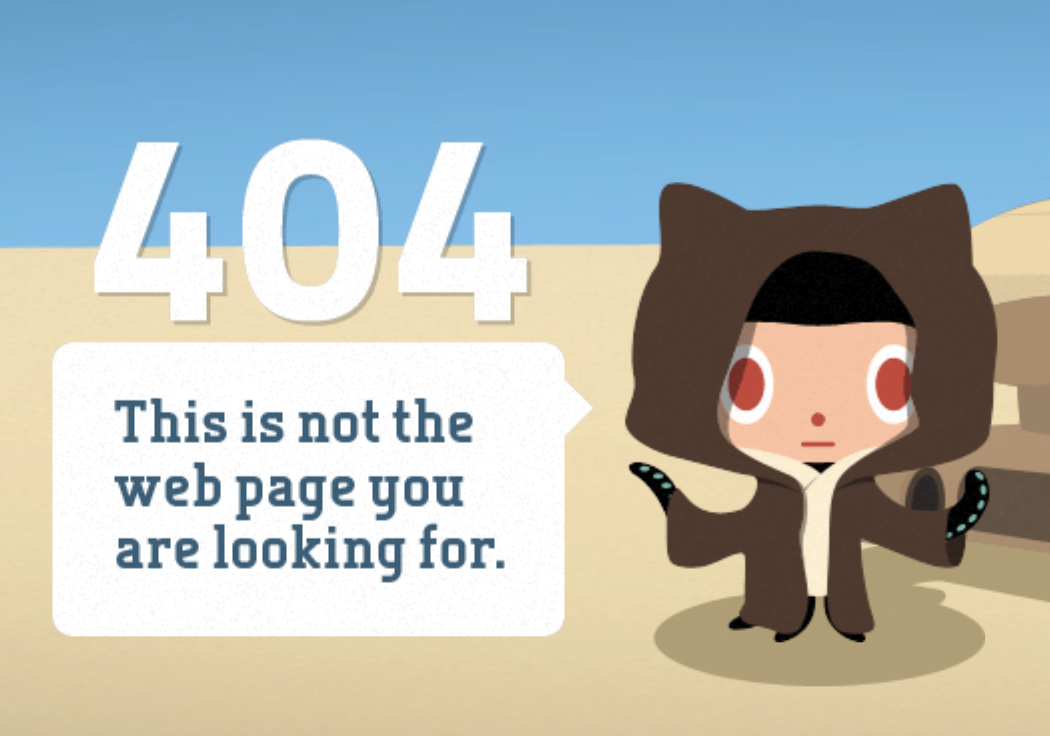
\includegraphics{404.png}
%     \caption[Google's 404 page]{Google's 404 page}
% \end{marginfigure}

% \marginpar{%
%   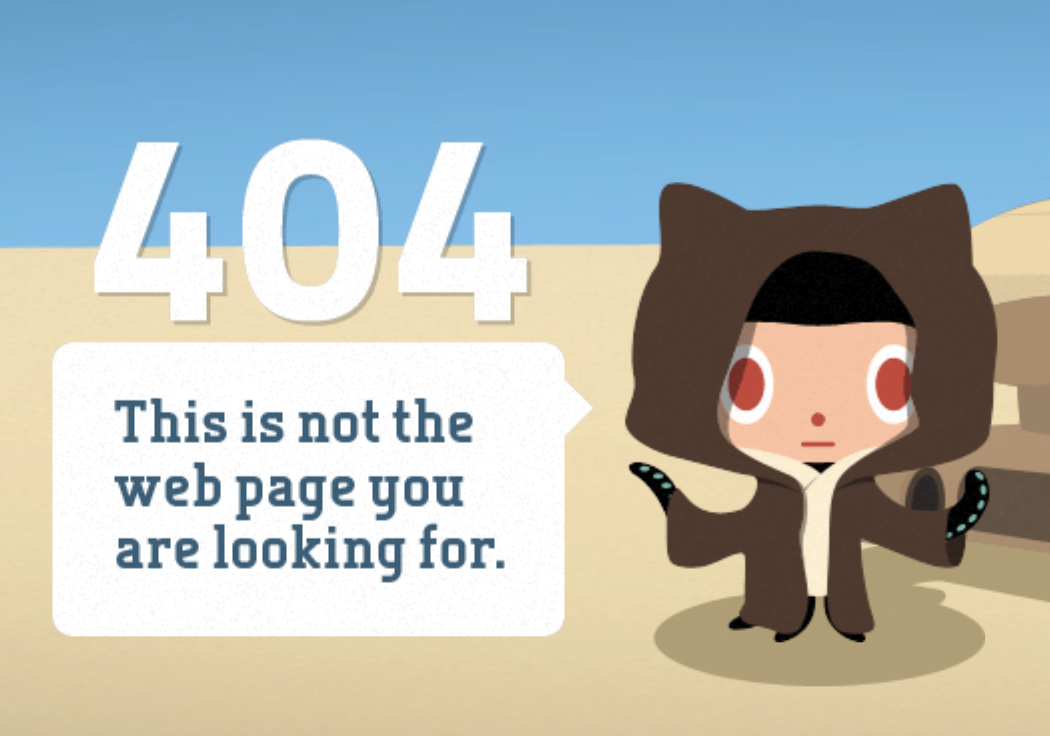
\includegraphics[width=\marginparwidth]{404.png}
%   \captionof{figure}{GitHub's 404 page}
% }
\margingraphic{404.png}{GitHub's 404 page}

You don't have to memorize these, but you'll find that after working with HTTP requests for a while they'll just come naturally. For example, you might be familiar with the infamous code \texttt{404}, which indicates that a resource was not found. You'll come to recognize other codes just like this one.

\begin{kaobox}[title=About the HTML we saw before\dots]
    What was it doing there? It's known as the \kw{body} of the response, and it's being sent back to the client, in essence, because that's what they asked for. Let's break things down. The client sent a \texttt{GET} request, asking the server to send some data back from a particular location (www.example.com). The data that was sent was this HTML code... Do you see where this is going yet? \\ \\
    We know that HTML is used by browsers in order to render web pages, so our client can now successfully render the web page stored on the server. In essence, the client uses this HTTP request in order to receive the data necessary to render a web page! This process happens billions of times per day, and it is the back bone of the whole internet. The internet is built upon servers which store HTML, CSS, and Javascript and your browser uses HTTP requests to request them to be sent to you! Obviously, there's more to the internet than just this, and we could fill many books talking about it, but it's outside the scope of this workshop series. If you're interested take CS 118!
\end{kaobox}

HTML is not the only thing that can be placed in response bodies. In fact, just looking at the \texttt{Accept} section of our HTTP request we can see that images can be as well!

\begin{verbatim}
    Accept: text/html,application/xhtml+xml,application/xml;
    q=0.9,image/avif,image/webp,*/*;q=0.8
\end{verbatim}

Another common data format used in HTTP bodies is known as \kw{JSON}, or Javascript Object Notation. We'll discuss JSON more in detail once we actually see it in action, but for now it suffices to understand that it is a way to encode objects in Javascript as strings. For example, the following code block shows an object called \texttt{heck} and its corresponding JSON string representation:

\vspace{.5cm}

\begin{lstlisting}[language=Java]
    heck = {
        studentOrgRanking: 1,
        color: "#C960FF",
        rizz: 100,
        website: "https://hack.uclaacm.com"
    }

    {
        "studentOrgRanking": 1,
        "color": "#C960FF",
        "rizz": 100,
        "website": "https://hack.uclaacm.com"
    }
\end{lstlisting}

\margingraphic{hack-chad.png}{Rizz 100}

\section{Web API's: What's on the Menu?}

Now that our server and client have a common language, it's time to take things a step further. Let's revisit the restaurant analogy. How does the customer know what they're allowed to order? They can't just demand to be served whatever they want, because the restaurant might not be able to accommodate their request.\sidenote{Yes, there are exceptions, secret menus, etc. But let's be real. If you order off the secret menu, the staff hates you.} That's why every restaurant has a menu! There needs to be a way to let customers know what they can order. Clients and servers are much the same. There needs to be an understanding between them about what the server can do for the client, and this is accomplished using the \kw{API}, or Application Programming Interface. You may have heard this term before. It's another one of those nebulous phrases that gets thrown around a lot, but is rarely defined concretely.

In general, an API is just a way for two computer programs to interact with each other. Think of the customer at a restaurant as one program and the staff as another. The customer hasn't eaten in 16 hours and is craving a burrito with carnitas and guacamole.\sidenote{I am so hungry right now.} Using the menu (the API), the customer is able to enjoy the result of the staff's work and they don't need to attend 4 years of culinary school in order to do it! Put another way, the API allows us to interact with a blackbox and receive meaningful results. API's can be found everywhere in software engineering, but we will be creating more specialized API's called \kw{Web API's}.\sidenote{As the name implies, these are API's that utilize the Web, allowing communication from client to server through HTTP requests.}

\begin{kaobox}[title=Let's take a look at an example of a simple API.]
    
    API's can be expressed in several ways, either using code or English. Let's keep it simple and just use English. Consider a server with the sole purpose being to simulate a cat. The API defines several actions that you, as a pet owner, can take to interact with the cat, and in response the server will send a JSON string (recall that JSON is just a string representation of a Javascript object) with information about the cat and its actions. \\

    The API is defined as follows:
    \begin{verbatim}
    POST FEED: You feed the cat.
    POST WATER: You give the cat a drink.
    POST PET: You pet the cat.
    GET STATUS: You check how the cat is doing.
    POST MEOW: You meow at the cat.
    \end{verbatim}

    These five actions define how you can interact with the cat server. Some of the interactions may have side effects, or an effect on the state of the cat. Also, notice the HTTP method names before each action name! Let's start by petting the cat. Note that the formatting below does not follow HTTP.

    \begin{verbatim}
    REQUEST: POST PET

    RESPONSE: 
    {
        "health": 100,
        "hunger": 10,
        "thirst": 10,
        "action": "Meows and sits down, ready 
                    for more pets."
    }
    \end{verbatim}

    He seems friendly! Let's give him some food.

    \begin{verbatim}
    REQUEST: POST FEED

    RESPONSE: 
    {
        "health": 100,
        "hunger": 50,
        "thirst": 10,
        "action": "Meows gratefully, 
                and attacks the food."
    }
    \end{verbatim}

    Okay, he seems to be enjoying that. Let's pet some more.
    \begin{verbatim}
    REQUEST: POST PET

    RESPONSE: 
    {
        "health": 100,
        "hunger": 50,
        "thirst": 10,
        "action": "Bites your hand. He wasn't 
            done eating yet!"
    }
    \end{verbatim}

    Ouch. How to respond?

    \begin{verbatim}
    REQUEST: POST MEOW

    RESPONSE: 
    {
        "health": 100,
        "hunger": 50,
        "thirst": 10,
        "action": "Looks up from food, confused."
    }
    \end{verbatim}

    Okay, that's enough playing with the cat! Hopefully, this toy example gave you a clearer idea of what an API is as well as its purpose. We'll be creating a real API later in this chapter using Javascript.

\end{kaobox}

Typically, Web API's contain multiple \kw{endpoints}. In general, an endpoint can be thought of as a point of contact between a client and a server. Depending on which endpoint is invoked, the server knows which action to take. In the previous example, we can think of each of the possible five actions as an endpoint. Another common way of thinking about endpoints is as \emph{specific digital locations} of resources located on a server. For example, if we want to access the resource located at \texttt{/MEOW} on a server, we use the \texttt{MEOW} endpoint. You can think about endpoints in whichever way is best for your own mental model, as long as you remember that endpoints are meant to direct the server towards a particular action or resource. And don't worry if things aren't clear yet! We'll be showing concrete examples of all of these concepts in the next few sections.

\margingraphic{kevin.jpg}{This is the cat. His name is Kevin.}

\section{Server Implementations}

As one might expect, there are many ways to go about implementing a server. We know that a server is simply a computer tasked with listening and responding to requests, and clearly this task is not specific to any single programming language. Some popular choices are the following:

\begin{itemize}
    \item Node.js and Express
    \item Python and Django
    \item Python and Flask
    \item C and Pain\sidenote{Pain in the literal sense of the word. Not recommended.}
\end{itemize}

There are countless libraries out there, so no need to reinvent the wheel. Since we're focusing on the MERN stack for Stackschool, we'll be going with Express and Node.\sidenote{Representing the E and N in MERN respectively.} To avoid any confusion let's first discuss what exactly they do, and why they are useful for us when building a server app.

\subsection*{What is Node?}

Originally, Javascript was created as a scripting language for the browser, Netscape, and wasn't intended to be executed outside of that environment.\sidenote{It also took only 10 days for the first version to be developed, which honestly explains a lot.} However, as time has gone on and Javascript has gotten more popular, it has transcended this original functionality. In 2009, a man named Ryan Dahl decided that Javascript would be an excellent language for writing server programs, and created a new runtime environment\sidenote{By runtime environment, I just mean a program that can execute code.} for it outside of the browser. Node was the product of his efforts. Now, years later, it's the most popular non-browser runtime for Javascript and home to a thriving, community driven ecosystem of libraries.\sidenote{We call these libraries packages, and we access them using a program called NPM, or Node Package Manager. Another popular (and, in my opinion, better) package manager is Yarn. We'll be using Yarn for all examples here.} As described on their website, Node is "an asynchronous event-driven JavaScript runtime designed to build scalable network applications." Essentially, it's perfect for servers!

\subsection*{What is Express?}

Node gives you all the fundamentals required to make a server, but why do that if someone's already done most of the work for us? Express is a framework that makes creating server applications far easier by abstracting away most of the HTTP request logic. There are plenty of alternative frameworks, but to stay true to the MERN stack, we'll be going with Express.

\subsection*{Creating Your First Server}

Now that we have all that out of the way, let's get to the fun part. First, make sure you have all the necessary installations. Follow the checklist:

\begin{itemize}
    \item Node. \href{https://nodejs.org/en/download/package-manager/#macos}{Here} is an extensive guide to installing no matter which platform you're on. I recommend using Homebrew if you're on MacOS.\sidenote{Some would recommend using a version manager like NVM, but if you just want to get your hands dirty quickly, the other methods are adequate for now.}
    \item Yarn. This will be your package manager, or the program you use to install node packages (like Express). Once you have Node installed, you can install Yarn by running \texttt{npm install -{}-global yarn} in your shell. 
\end{itemize}

Now in your terminal, navigate to the directory of your choice\sidenote{If you're not familiar with navigating the terminal, check out \href{https://www.digitalocean.com/community/tutorials/basic-linux-navigation-and-file-management}{this} resource.} and run \texttt{yarn init}. This will start the process of creating your server application. It'll prompt you with some basic configuration information, but you can just accept the default values by pressing enter for each one. Don't worry, you can change these values later! After you've completed this step, a new file called \texttt{package.json} should have been generated. This is the configuration file for your server. To install Express, run \texttt{yarn add express}. This should generate a directory called \texttt{node\_modules} and a file called \texttt{yarn.lock}.

Now let's make the server itself. Create a new file called \texttt{server.js}. Within this file, add this boilerplate code:

\begin{lstlisting}[language=Java]
    /**** INIT SERVER ****/
    const express = require('express');
    const app = express();
    app.use(express.json());
    
    /**** DEPLOY SERVER ****/
    const port = 8080;
    
    app.listen(port);
    console.log(`listening on http://localhost:${port}/`);
    console.log("Press Ctrl-C to quit");
\end{lstlisting}

Congrats, you just made your first server! Unfortunately, it doesn't do anything. You can run it with \texttt{node server.js}. Before making it a bit more useful, let's break down what exactly is happening. Take a look at the second line. In Node, the \texttt{require} function is a way to include code from other files within your file.\sidenote{Similar to imports/includes in other languages you may be familiar with. We call the code that we're importing a "module."} In this case, we're including code from the Express package. In the next line, we create an Express app and bind it to a variable. In the final stage of initialization, we tell the app to use something called a \kw{middleware} function. We'll get into these in more detail soon, but for now just know that it's a way to make your life easier. Now, in the deployment section, we define a port, and tell the server to listen on that port. This will affect the URL of your local server.

Alright, now that we've cleared all that up,\sidenote{May be worth a couple more readthroughs if it's still unclear, or get in contact with us on \href{https://discord.gg/xXcJWDUqJj}{Discord}!} its time to add our first endpoint. We'll make an endpoint that requests a random number from the server. It's pretty easy!

\begin{lstlisting}[language=Java,firstnumber=6]
    /**** ROUTES ****/
    app.get("/random", (req, res) => {
        // generate random number from 1-100
        const rand = Math.floor(Math.random() * 100) + 1;

        // send random number in response
        res.send(`${rand}`);
})
\end{lstlisting}

This endpoint can be referred to as \texttt{GET /random}\sidenote{Note that \texttt{/random} is referred to as a \kw{route}. The distinction between endpoints and routes is that endpoints include the HTTP method (i.e. GET, POST, etc.) in their definition. You can have multiple endpoints with the same route, as long as the method is different (so having \texttt{GET /random} and \texttt{POST /random} would be perfectly fine).} and every time it is invoked it will return a string containing a random number from 1-100. You can test it out by starting the server and visiting \url{http://localhost:8080/random} in your browser.\sidenote{In order to start your server, use \texttt{node server.js}.} At a surface level, all that's going on here is that we're using Javascript code to define our server's API. 

\begin{kaobox}[title=Describing the API with English]
    Recall how we defined our API in the cat server example. We can describe our Javascript endpoint definition for random in the same way! 

    \begin{verbatim}
    GET /random: Get a random number from 1-100.
    \end{verbatim}
    
    They're two ways of saying the same thing, except that one of them happens to be real, functional code.
\end{kaobox}

Hopefully, you now have a feel for the general process of creating Express applications. You're now ready to put everything together into a more realistic application.

\section{Demo}

\section{Testing}

\section{Organization}